%%
%% This is file `./samples/longsample.tex',
%% generated with the docstrip utility.
%%
%% The original source files were:
%%
%% apa7.dtx  (with options: `longsample')
%% ----------------------------------------------------------------------
%% 
%% apa7 - A LaTeX class for formatting documents in compliance with the
%% American Psychological Association's Publication Manual, 7th edition
%% 
%% Copyright (C) 2021 by Daniel A. Weiss <daniel.weiss.led at gmail.com>
%% 
%% This work may be distributed and/or modified under the
%% conditions of the LaTeX Project Public License (LPPL), either
%% version 1.3c of this license or (at your option) any later
%% version.  The latest version of this license is in the file:
%% 
%% http://www.latex-project.org/lppl.txt
%% 
%% Users may freely modify these files without permission, as long as the
%% copyright line and this statement are maintained intact.
%% 
%% This work is not endorsed by, affiliated with, or probably even known
%% by, the American Psychological Association.
%% 
%% ----------------------------------------------------------------------
%% 
\documentclass[man]{apa7}

\usepackage{lipsum}

\usepackage[american]{babel}

\usepackage{caption} % For captioning outside figures
\usepackage{capt-of} % For captioning outside figures

\usepackage{csquotes}
\usepackage[style=apa,backend=biber]{biblatex}
\addbibresource{bibliography.bib}

\title{Laser Scanning Comparison Using CloudCompare}
\shorttitle{}
\authorsnames{Jule Valendo Halim -1425567}
\authorsaffiliations{GEOM90038 - Advanced Imaging}

\begin{document}
\maketitle
\vspace{-6em}
\section{Introduction\vspace{-5em}}

Light detection and ranging (LiDAR) sensor consists of a transmitter and a receiver. The transmitter contains a laser that emits beams of light, while the receiver collects the photons that return from the transmitted laser (\Textcite{wandinger2005}). Figure \ref{fig:lidarSetup} shows a simple representation of a LiDAR system.

\begin{minipage}{\linewidth}
  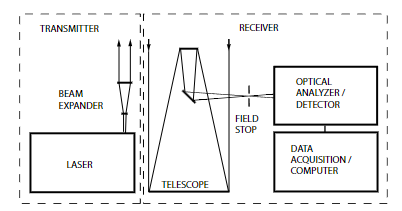
\includegraphics[bb=0in 0in 2.5in 2.5in, height=2.5in, width=2.5in]{figures/lidarSetup.png}
  \captionof{figure}{Principle setup of a LiDAR system (\Textcite{wandinger2005})}
  \label{fig:lidarSetup}
\end{minipage}

Multiple forms of LiDAR systems can be used for various applications. For example, \Textcite{conti2024} compared two applications of LiDAR sensors in the use of an Italian town hall building. The two sensor applications are terrestrial and mobile laser scanners (TLS and MLS respectively). A terrestrial laser scanner uses a LiDAR sensor mounted on a tripod and scans the area around it. The TLS is able to capture a wide area through a mirror within the hardware that can rotate and reflect the lasers in many angles. Meanwhile, the MLS is a handheld LiDAR sensor that can be carried and transported with one hand. Capturing wider areas with this device is possible due to the handheld nature, where a user would move around and capture the entire area. Figure \ref{fig:TLSandMLS} shows a MLS and TLS device.

\begin{minipage}{\linewidth}
  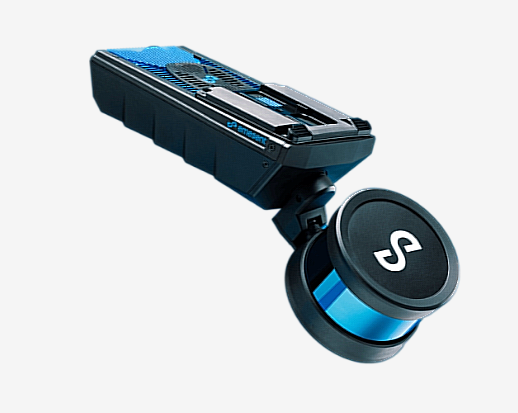
\includegraphics[height=\textheight/3,width=\textwidth/2]{figures/HoverMap.png}
  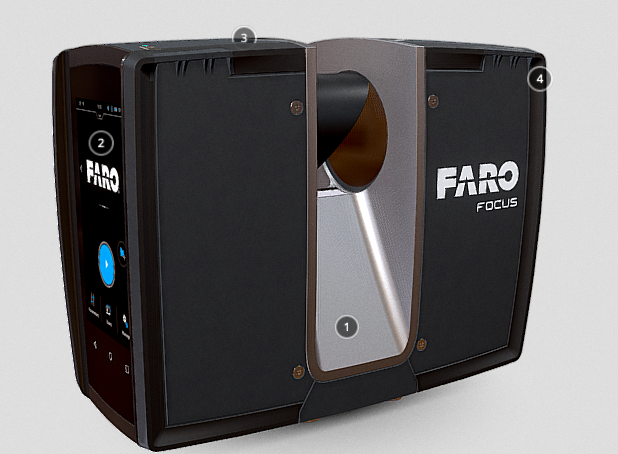
\includegraphics[height=\textheight/3,width=\textwidth/2]{figures/FaroFocus.png}
  \captionof{figure}{Hovermap Emesent MLS (left) (\Textcite{emesent}) and FAROFocus TLS (right) (\Textcite{FARO})}
  \label{fig:TLSandMLS}
\end{minipage}

\Textcite{conti2024} found that the MLS is able to create a streamlined and efficient workflow that is suitable for the documentation of heritage buildings. However, where a higher level of detail is required, the TLS would be more suitable. In this report, I aim to investigate the differences in the MLS and TLS through using the LiDAR systems shown in figure 2. Dense point clouds will be obtained for each system before being compared using the open source software CloudCompare. This software has been shown to be able to compare two different point clouds and investigate their respective quality (\Textcite{girardeau2016}). 

The overall procedure in investigating both LiDAR systems involves with firstly determining hardware settings and object to be scanned, followed by performing the scan to create a dense point cloud. The resulting point clouds will then be aligned and compared to each other qualitative and quantitatively. More details regarding the project procedure will be discussed in the methods section.

\section{Method}

\subsection{Initial Settings}

For the remainder of the report, the MLS will refer to the Hovermap Emesent and the TLS will refer to the FAROFocus.

Initial settings were set to capture an indoor area with a range of 10m (ie., the room boundaries are within 10m of the TLS). The TLS was also configured to capture images using colour. Afterwards, the resolution and quality settings are set to 1/5 and 4x respectively. The resolution indicates that one in every 5 points would be scanned, and the quality indicates that each of these scans would occur 4 times. Additional setting for the TLS such as the pixel dimensions of each scan and time taken 
for the scan can be seen in figure \ref{fig:TLSSettings}.

\begin{minipage}{\linewidth}
  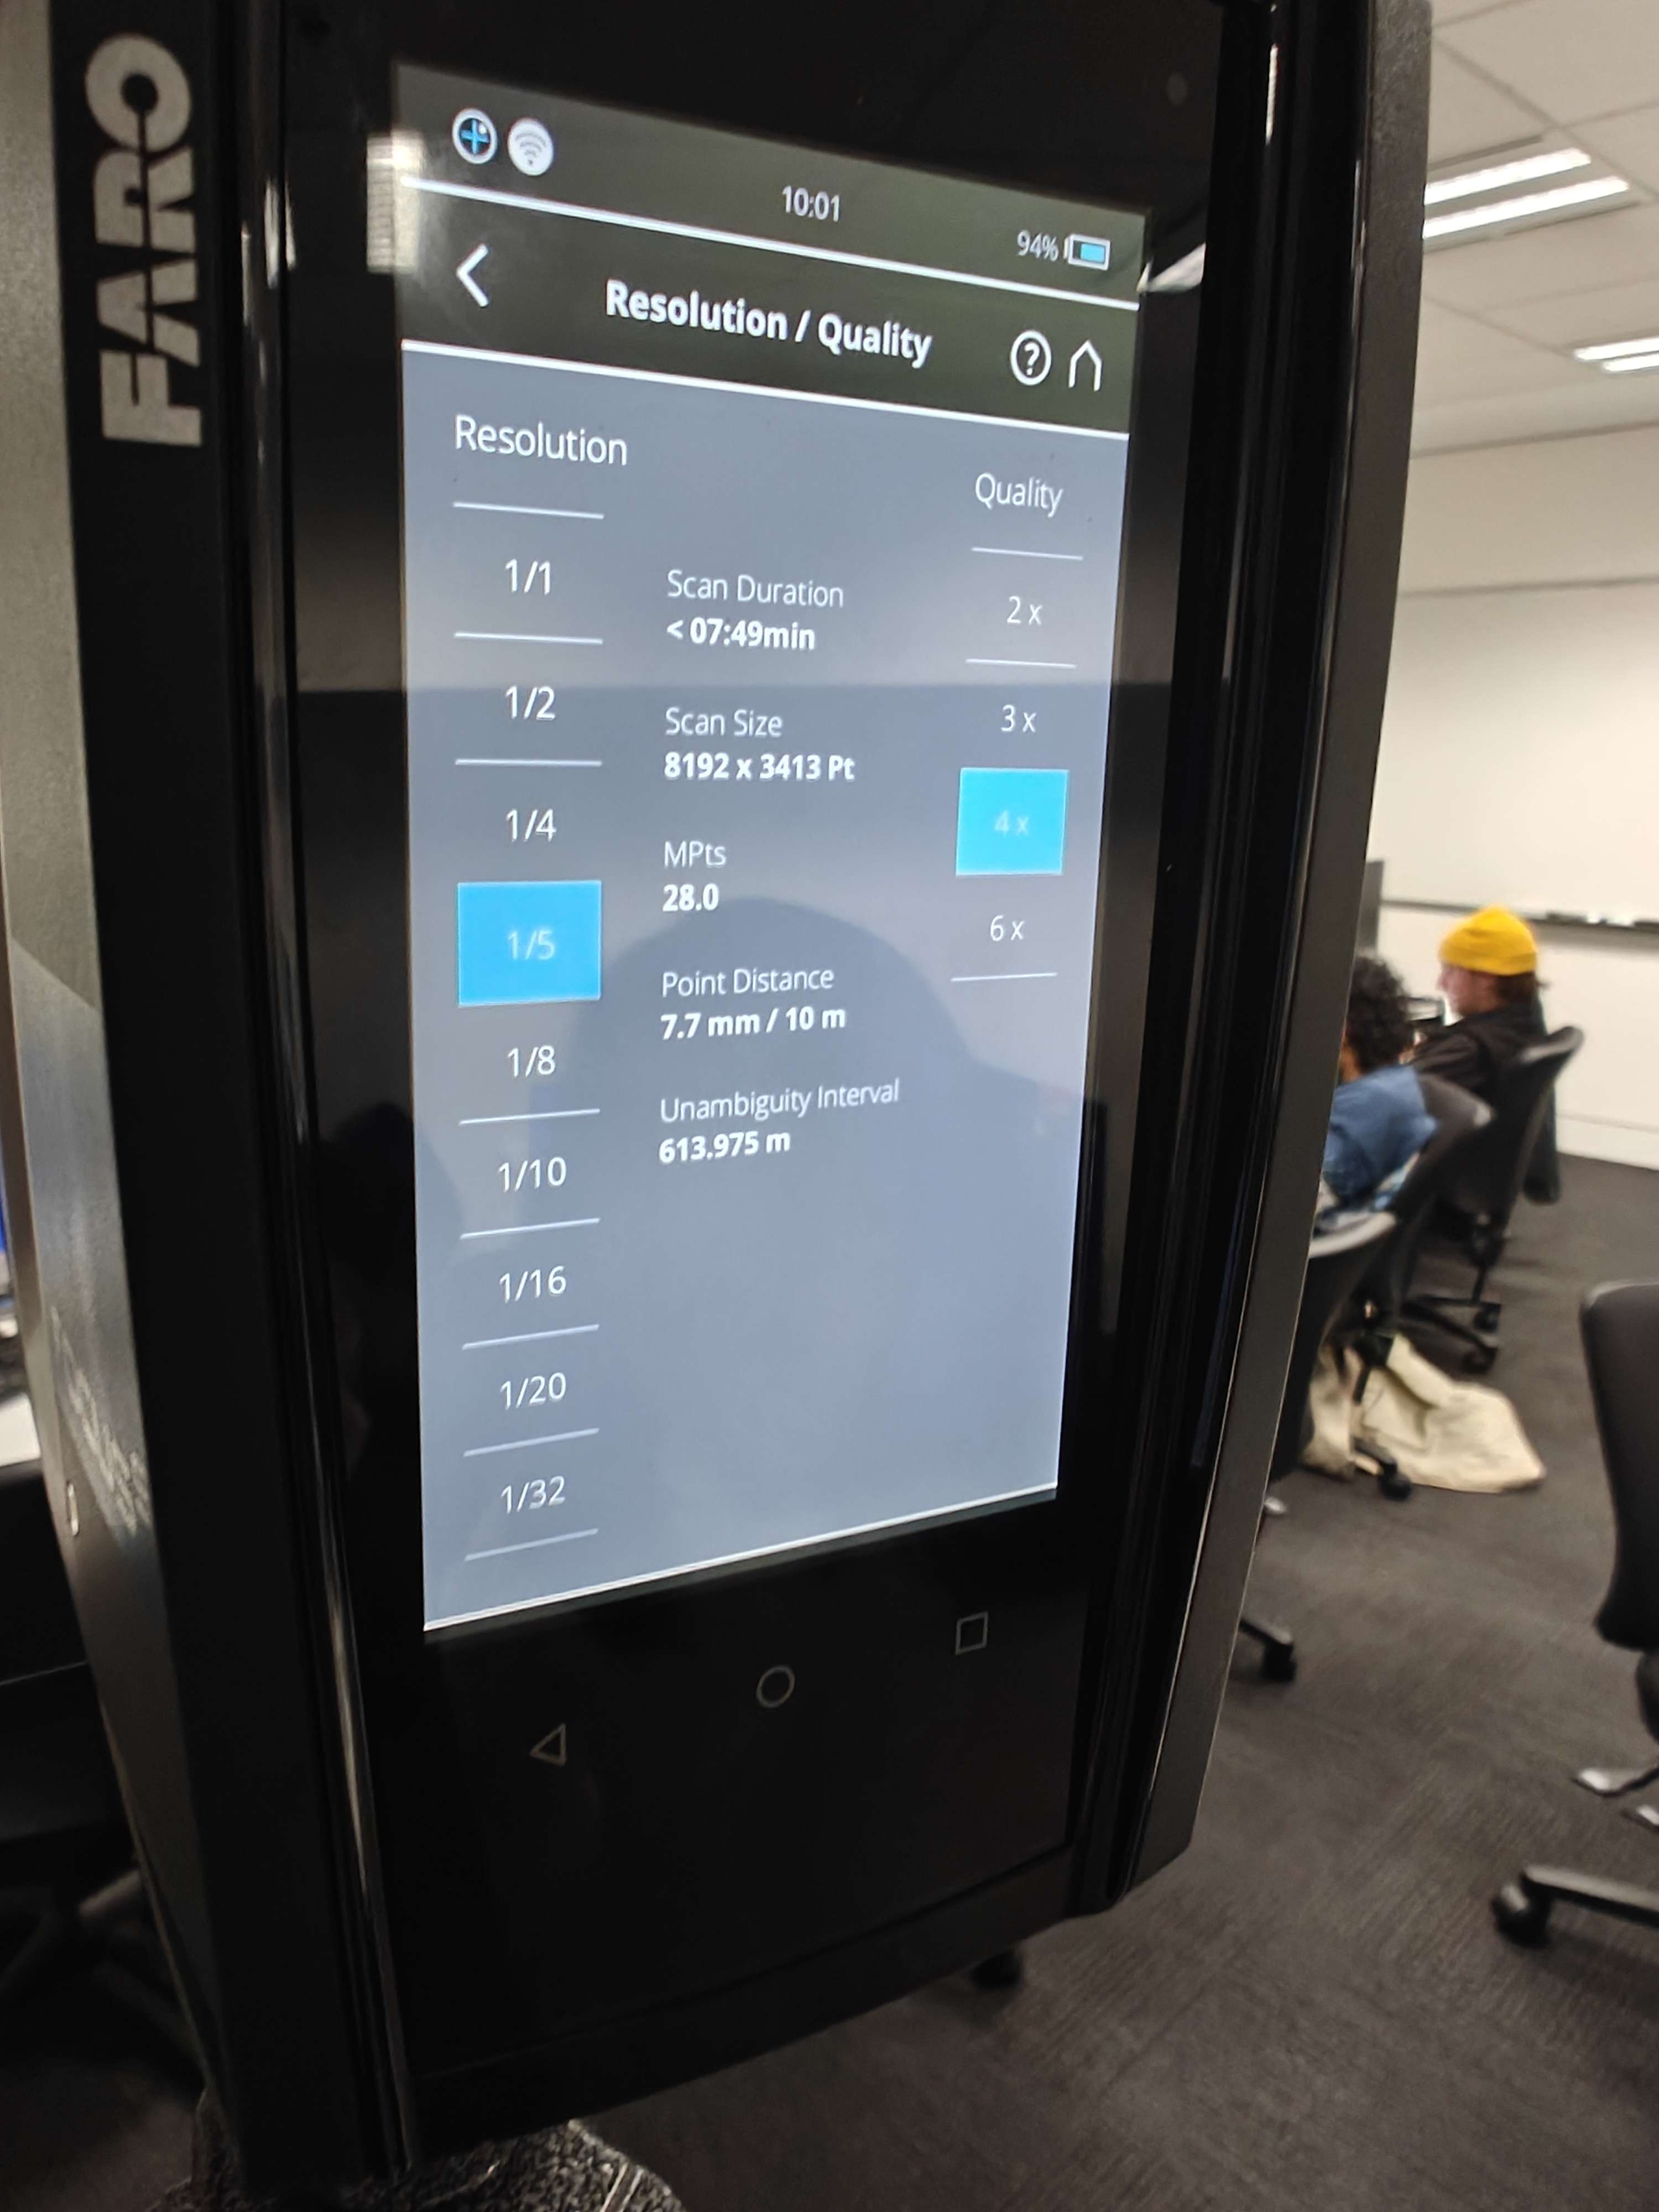
\includegraphics[height=\textheight/2 ,width=\textwidth/2]{figures/IMG20240418194000.jpg}
  \captionof{figure}{Settings for the TLS}
  \label{fig:TLSSettings}
\end{minipage}

The MLS was first connected to its mobile app. After this connection is established, the app can be used to control its operation (ie., starting and stopping its scan.)


\subsection{TLS and MLS Point Cloud Alignment}

\subsubsection{Manual Alignment}
Both point clouds were added to the CloudCompare workingspace. Using the rotation and trasnlation tools, the MLS point cloud was carefully oriented to overlap with the orientation and position in space of the TLS. Figure \ref{fig:manualAlignment} shows the difference of orientation after manual alignment. The grey point clouds are from the MLS, while the point cloud with more colour is from the TLS.

\begin{minipage}{\linewidth}
  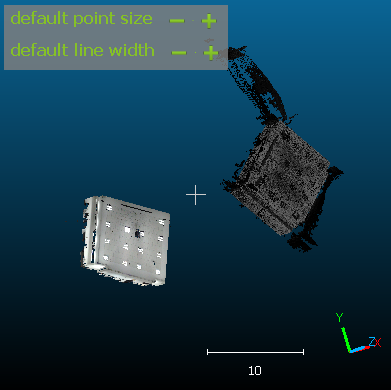
\includegraphics[height=\textheight/3,width=\textwidth/2]{figures/InitialAlignments.png}
  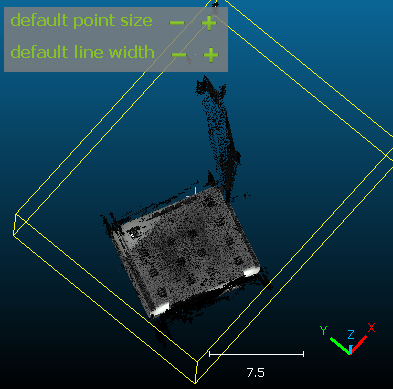
\includegraphics[height=\textheight/3,width=\textwidth/2]{figures/FinalAlignments.png}
  \captionof{figure}{Inital alignments when point clouds were added (left) and the result of manual alignment (right)}
  \label{fig:manualAlignment}
\end{minipage}

Visual inspection was done at this stage to identify whether or not each point cloud appeared to be aligned. Afterwards, coarse and fine registration was used to identify the errors in alignment.

\subsubsection{Coarse and Fine Registrations}
Coarse registration is done by using the align (point pairs picking) tool in CloudCompare. This tool performs references one point cloud to the other using reference points selected manually. A total of 6 (3 in each point cloud) reference points were selected. The MLS is the to-be-aligned entity, while the TLS was the reference point cloud.

Afterwards, fine registration was performed. This process involved using the fine registration (ICP) tool from CloudCompare. Fine registration is only possible after coarse registration. Again, the TLS was the reference point and the MLS was the reference point cloud. 

For both registrations, the RMSE and transformation matrices were recorded after registration was completed.

\subsection{Cloud to Cloud Distance}

\section{Results}
Table~\ref{tab:BasicTable} summarizes the data. \lipsum[1-3]
\vspace{20pt}

\begin{minipage}{\linewidth}
  \captionof{table}{Sample Basic Table}
  \label{tab:BasicTable}
  \begin{tabular}{@{}llr@{}}         \toprule
  \multicolumn{2}{c}{Item}        \\ \cmidrule(r){1-2}
  Animal    & Description & Price \\ \midrule
  Gnat      & per gram    & 13.65 \\
            & each        &  0.01 \\
  Gnu       & stuffed     & 92.50 \\
  Emu       & stuffed     & 33.33 \\
  Armadillo & frozen      &  8.99 \\ \bottomrule
  \end{tabular}
\end{minipage}

\vspace{20pt}

\lipsum[1]

Figure~\ref{fig:Figure1} shows this trend.

\vspace{20pt}
\begin{minipage}{\linewidth}
  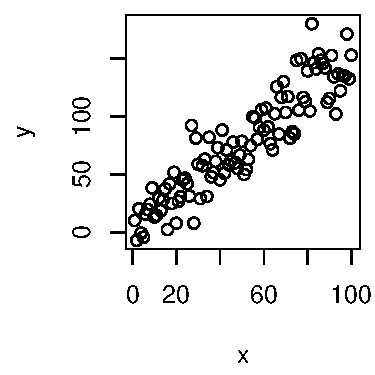
\includegraphics[bb=0in 0in 2.5in 2.5in, height=2.5in, width=2.5in]{figures/Figure1.pdf}
  \captionof{figure}{This is my first figure caption.}
  \label{fig:Figure1}
\end{minipage}

\section{Discussion}
\lipsum[17]

\lipsum[18]

\lipsum[19]

\printbibliography


\end{document}

%% 
%% Copyright (C) 2021 by Daniel A. Weiss <daniel.weiss.led at gmail.com>
%% 
%% This work may be distributed and/or modified under the
%% conditions of the LaTeX Project Public License (LPPL), either
%% version 1.3c of this license or (at your option) any later
%% version.  The latest version of this license is in the file:
%% 
%% http://www.latex-project.org/lppl.txt
%% 
%% Users may freely modify these files without permission, as long as the
%% copyright line and this statement are maintained intact.
%% 
%% This work is not endorsed by, affiliated with, or probably even known
%% by, the American Psychological Association.
%% 
%% 
%% This work is "maintained" (as per LPPL maintenance status) by
%% Daniel A. Weiss.
%% 
%% This work consists of the file  apa7.dtx
%% and the derived files           apa7.ins,
%%                                 apa7.cls,
%%                                 apa7.pdf,
%%                                 README,
%%                                 APA7american.txt,
%%                                 APA7british.txt,
%%                                 APA7dutch.txt,
%%                                 APA7english.txt,
%%                                 APA7french.txt,
%%                                 APA7german.txt,
%%                                 APA7ngerman.txt,
%%                                 APA7greek.txt,
%%                                 APA7czech.txt,
%%                                 APA7turkish.txt,
%%                                 APA7endfloat.cfg,
%%                                 Figure1.pdf,
%%                                 shortsample.tex,
%%                                 longsample.tex, and
%%                                 bibliography.bib.
%% 
%%
%% End of file `./samples/longsample.tex'.
